\section{Aprendizado de Máquina}
\label{cap:2.2}

É possível notar que, nos últimos anos, houve um expressivo aumento do uso de técnicas de inteligência artificial (do inglês, \textit{artificial intelligence}, AI) e de aprendizado de máquina (do inglês, \textit{machine learning}, ML) em diversas áreas da computação. Uma das grandes vantagens de utilizar técnicas de aprendizado de máquina é garantir que associações entre variáveis independentes possam ser encontradas de forma dinâmica, sem depender de instruções humanas explícitas \citet{bib:livroRaschka}. Estratégias de ML para aprender com dados disponíveis são benéficas para a solução de problemas, principalmente quando estes possuem grande volume de dados, como é o caso da codificação de vídeo. Quanto maior a quantidade e a variedade de informações disponíveis para tomada de decisão, maior é a dificuldade de encontrar relações úteis utilizando apenas a estatística e isso pode ser contornado com o uso de modelos de aprendizado de máquina.

Conforme descrito em \citet{bib:livroRaschka}, o uso de modelos de aprendizado de máquina é possível seguindo alguns passos facilmente identificáveis em quatro fases principais, como bem exemplificado na Figura \ref{fig:6}: 

\begin{figure}
    \centering
    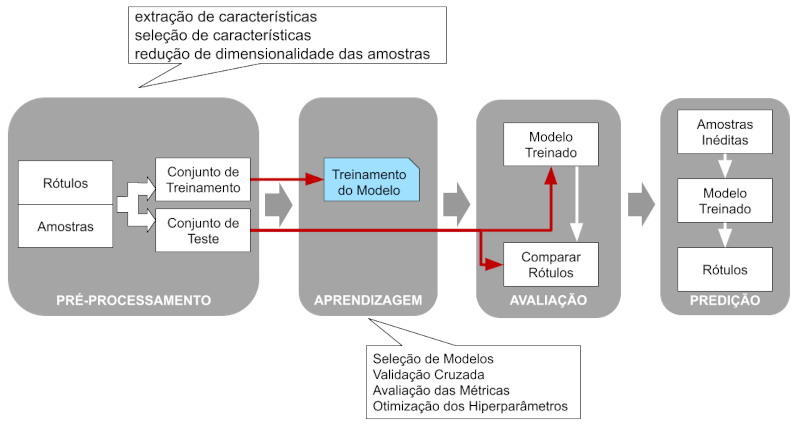
\includegraphics[width=\textwidth]{FIGURES/fig_6.png}
    \caption{Fases da vida de um modelo de aprendizado de máquina supervisionado. Fonte: Elaborada pelo autor com base em \citet{bib:livroRaschka}.}
    \label{fig:6}
\end{figure}

\begin{enumerate}[(i)]
    \item pré-processamento de dados;

    \item aprendizado;

    \item validação dos resultados;

    \item predição.
\end{enumerate}

É na primeira fase em que ocorre a extração dos dados brutos e a preparação destes para serem processados pelo algoritmo de ML. Esses dados dificilmente oferecem algum tipo de informação útil para que um modelo consiga gerar conhecimento; é necessário lapidá-los de forma a possibilitar que informações padronizadas sejam extraídas deles. Por essa razão, esta fase tende a ser uma das mais custosas de todo o ciclo de vida do uso de um modelo de aprendizado de máquina. Após a finalização da organização dos dados é que poderemos dividi-los em subconjuntos úteis para as demais fases: 

\begin{enumerate}[(a)]
    \item dados de treinamento;

    \item dados de teste;

    \item dados de validação.
\end{enumerate}

O primeiro subconjunto de dados é particularmente importante, pois é com ele que alimentamos o treinamento do modelo de aprendizado de máquina (fase (ii) do ciclo de vida). Neste conjunto, constam todos os dados válidos para treinamento (denominados atributos) e a respectiva resposta esperada para esses dados (também denominado rótulo). O segundo subconjunto é utilizado para verificar o quanto o modelo aprendeu com os dados de treinamento (fase (iii) do ciclo de vida). Basicamente, expõe-se o modelo aos dados de entrada inéditos e comparam-se os resultados de saída com os esperados para aqueles conjuntos de dados de entrada, possibilitando que se calcule a confiabilidade do modelo. É particularmente importante que os dados de treinamento e de teste sejam diferentes, afinal estamos utilizando um modelo de aprendizado de máquina para solucionar problemas desconhecidos, e não para explorar o que ele já conhece. Outro subconjunto de dados que pode ser utilizado é o de validação. Este é essencialmente similar ao subconjunto de dados de testes, só que com uma menor quantidade de dados, usados principalmente para verificar e ajustar os hiperparâmetros do modelo (explicaremos nos próximos parágrafos), quando necessário. O subconjunto de dados de validação é empregado interativamente com o conjunto de dados de treinamento, ainda na fase (ii) do ciclo de vida. Por fim, a fase (iv) do ciclo de vida é, em essência, a aplicação do modelo a situações reais, nas quais não há conhecimento prévio das saídas esperadas.

Há diversos algoritmos de aprendizado de máquina, classificados de acordo com sua forma de aprendizado \cite{bib:livroML} \cite{bib:livroKubat}. No \textbf{Aprendizado Supervisionado}, o resultado esperado (seja um dado categórico, seja um dado numérico) é conhecido e faz parte do conjunto de dados utilizados no processo de treinamento, conforme exemplos de dados apresentados anteriormente. Por outro lado, quando não há um resultado esperado ou quando este não é conhecido previamente ao processo de treinamento, empregam-se os modelos de \textbf{Aprendizado Não-Supervisionado}, cujo objetivo principal consiste justamente em encontrar as categorias ou valores que definem os dados de entrada, sendo especialmente útil para quando o objetivo do modelo é explorar os dados a fim de descobrir informações não óbvias. Por fim, há os modelos de \textbf{Aprendizado por Reforço}, em que o algoritmo aprende com os dados e se ajusta reiteradamente, utilizando mecanismos para atribuir penalidades (de modo a minimizar o erro) e recompensas (de modo a maximizar os acertos) ao longo das interações; isso possibilita que o modelo seja capaz de tomar decisões cada vez melhores, dentro de um ambiente dinâmico.

Sendo assim, quando observamos as classificações de aprendizado de máquina, conforme sua forma de aprendizado, e uma possível aplicação desses modelos em codificadores de vídeo, intuitivamente supomos que os modelos de aprendizado supervisionado sejam utilizados, uma vez que as decisões que podem ser tomadas já são conhecidas. Ou seja, apesar da elevada complexidade de um codificador de vídeo, as diversas etapas que o compõem possuem um rol limitado de opções de escolha; logo, modelos de aprendizado supervisionado são os mais adequados a esse contexto. Isso não significa que os demais algoritmos de aprendizado de máquina não possam ser aplicados a codificadores de vídeo, apenas que é menos comum.

Por fim, cabe definir o termo hiperparâmetro, que será utilizado nas próximas seções. Os hiperparâmetros são utilizados para configurar o funcionamento de algoritmos de aprendizado de máquina, tornando possível a geração de diferentes modelos preditivos com os mesmos dados de entrada. Cada algoritmo de aprendizado de máquina possui um conjunto de hiperparâmetros que podem ser configurados, como, por exemplo,a profundidade máxima das árvores treinadas em algoritmos do tipo árvore de decisão. Existe um grande número de hiperparâmetros que podem ser configurados em cada algoritmo e cada conjunto de configurações de hiperparâmetros é denominado combinação de hiperparâmetros. Alguns autores denominam essa combinação de hiperparâmetros como combinação candidata. Esta será também a nomenclatura adotada nas seções desta tese que tratam de soluções baseadas em aprendizado de máquina supervisionado.
